\Chapter{Az \texttt{OpenCL} nyelv}

Open Computing Language egy keretrendszer amely lehetőséget ad olyan programok írására amelyek különböző platformokon is futtathatóak.
Az \texttt{OpenCL} meghatároz egy programozási nyelvet az eszközök és API-k számára a platformok vezérléséhez és a számítások végrehajtásához az eszközökön. Szabványos interfészt biztosít a párhuzamos számításokhoz, melyekhez adatalapú és feladatalapú párhuzamosítást használ.

Fontos észrevenni, hogy az \texttt{OpenCL} natív módon képes beszélni az eszközök nagy részével, de ez nem azt jelenti, hogy a kód optimálisan fog futni. Ugyanis különböző \texttt{CL} eszközök különböző funkciókkal vannak ellátva. Gyártó specifikus kiterjesztések elkerülésével a kód hordozható lesz, de nem sebesség optimális.

\begin{figure}[h!]
\centering
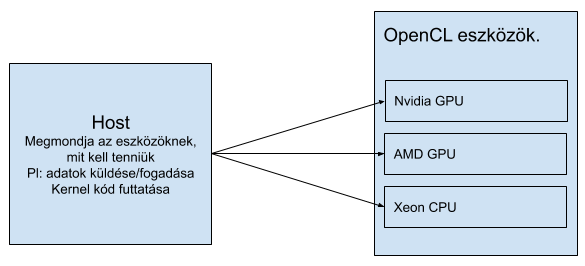
\includegraphics[width=12cm]{images/opencl.png}
\caption{\texttt{OpenCL}}
\label{fig:opencl}
\end{figure}

A következő esetekben a GPU-t érdemes használni:
\begin{itemize}
\item Gyors permutáció: Az eszközök gyorsabban mozgatáják a memóriát mint a Host.
\item Adat átváltás: Egyik formátumról másikra.
\item Numerikus gyorsítás: Az eszközök gyorsabban számolnak nagyobb adatdarabokkal mint a Host.
\end{itemize}
Jelen esetben a Host egy asztali számítógép.
Számítási eszközei: CPU, GPU, FPGA, DSP.
A számítási egységek: a magok száma
Elemek feldolgozása: ALU magonként.

\texttt{OpenCL} használata mellett szükségtelen gondolkozni azon, hogy pontosan mi is végzi el a számításokat. Ugyanis az \texttt{OpenCL} modelljének illeszkedése egy adott hardverhez, a gyártók feladata.

\begin{table}[h!]
\centering
\caption{CPU-k és GPU-k összehasonlítása}
\medskip
\label{tab:cpuvsgpu}
\begin{tabular}{|p{7cm}|p{7cm}|}
\hline
Alacsony számítási sűrűség & Magas számítási sűrűség \\
\hline
Komplex logikai vezérlő & Magas számítási és memória-hozzáférés \\
\hline
Nagy caches & Nincs nagyméretű gyorsítótár  \\
\hline
Optimalizált a soros műveletekre.
\begin{itemize}
	\item Kevesebb végrehajtási egység (ALU).
	\item Magas órajel sebesség.
\end{itemize} & Beépített párhuzamos műveletek.
\begin{itemize}
	\item Sok párhuzamos végrehajtási egység (ALU).
	\item A grafika a párhuzamosság legismertebb esete.
\end{itemize} \\
\hline
Keskeny adatvezeték <30 szakasz & Széles adatvezeték több száz szakasz \\
\hline
Alacsony késleltetési tolerancia & Magas áteresztőképesség, magas késleltetési tolerancia \\
\hline
Az újabb CPU-k több párhuzamosításra képesek & Újabb GPU-k
\begin{itemize}
	\item Jobb áramlást vezérlő logika
	\item Scatter/Gather Memory Access
	\item Már nem egyirányúak a pipeline-ok
\end{itemize} \\
\hline
\end{tabular}
\end{table}

\Section{Az OpenCL elemei}

\SubSection{Eszköz modell}

\begin{figure}[h!]
\centering
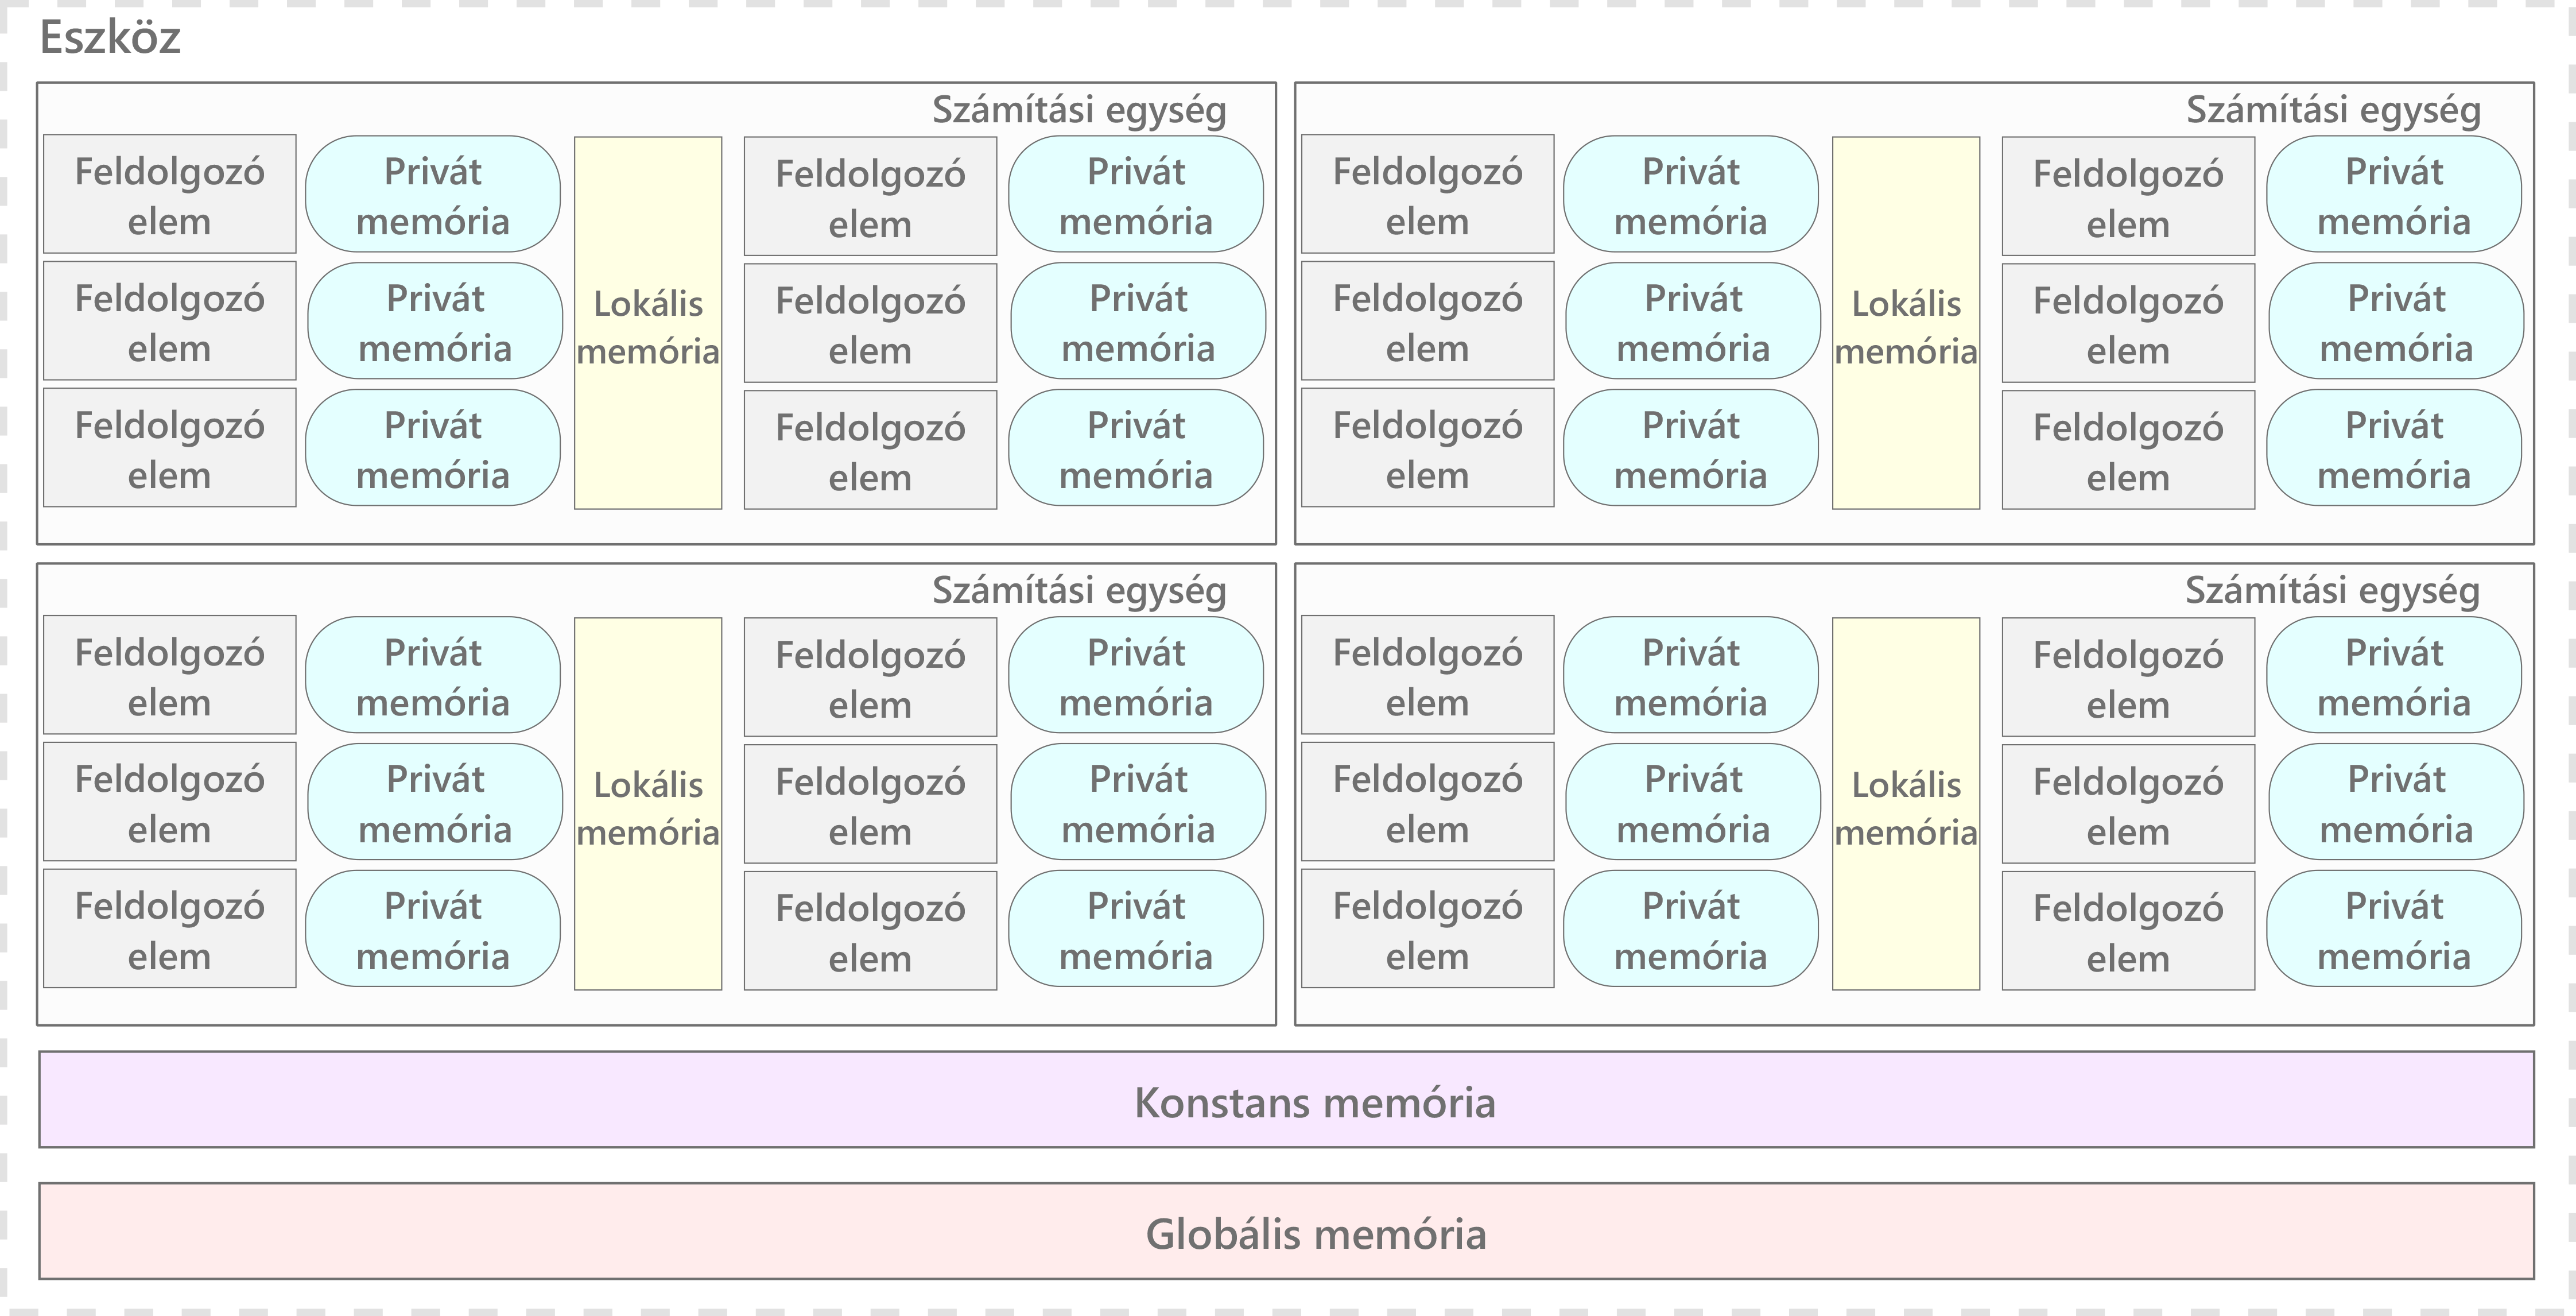
\includegraphics[width=\textwidth]{images/device.png}
\caption{\texttt{OpenCL} eszköz modell}
\label{fig:opencl}
\end{figure}

Négy féle memóriát különböztetünk meg:
\begin{itemize}
\item Globális memória: Minden eszközzel meg van osztva, de lassú. A kernel hívások között perzisztens. 
\item Konstans memória: Gyorsabb a globálisnál, szűrő paraméterek megadására használják.
\item Lokális memória: Minden számási egység számára privát, de megosztott a feldolgozó elemek között.
\item Privát memória: Gyorsabb a lokálisnál, minden feldolgozó elemnek van.
\end{itemize} 
A konstans, lokális és privát memóriába nem lehet adatokat menteni úgy, hogy más kernel használhassa majd azt.

\SubSection{Feldolgozási modell}

A Host -on \texttt{OpenCL} alkalmazások futnak amelyek a számítási eszközökhöz küldik a munkát.
\begin{itemize}
\item Munkaelem: A számítási eszköz alapvető egysége.
\item Kernel: A kód, ami fut a munkaegységen  (Alap C függvények)
\item Program: Kernelek és egyéb funkciók gyűjteménye
\item Kontextus: A környezet a munkaelemek végrehajtásához. (Eszközök, annak memóriái és parancssorai)
\item Parancssor: Sor melyet a Host arra használ, hogy a munkát (Kernelek, memória másolatok) az eszközbe küldje.
\end{itemize}

Ez egy keretrendszer, amely meghatározza, hogy a kernel hogyan hajtsa végre a probléma egyes pontjait. Vagy hogyan bontsa a feladatot munka elemekre.

Amire ehhez szükség van:
\begin{itemize}
\item Globális munkaméret. Ez általában egy bemeneti vektor teljes hossza.
\item Globális eltolás.
\item Munkacsoport méret.
\end{itemize}
Megfeleltetés:
\begin{itemize}
\item Munkaelem - számítási elem: Minden munkaelemet egy számítási elem hajt végre.
\item Munkacsoport - számítási egység: Minden munkacsoportot egy számítási egység hajt végre. A munkacsoport munkaelemek, a számítási egység pedig számítási elemek csoportja.
\item Kernel végrehajtási példány - Számítási eszköz. Munkacsoportok összessége illetve számítási elemek összessége. 
\end{itemize}

\SubSection{Munkacsoportok}

Ideális esetben végtelen számú feldolgozási elemmel rendelkezik az eszköz, Minden ilyen elem az adatok egy részét kezeli anélkül, hogy szükségük lenne kommunikációra. De ez a gyakorlatban nem szokott ilyen egyszerű lenni, ezért a munkát fel kell osztani.
\begin{itemize}
\item A teljes munkát fel kell osztani kisebb darabokra.
\item Minden darab egy munkacsoporthoz tartozik.
\item A munkacsoportokat ütemezéssel kell végrehajtani a számítási egységeken.
\item Minden csoport rendelkezik egy megosztott memóriával, ami olyan mint a lokális memória a számítási-egységeknél
\end{itemize}
A folytatáshoz a munkacsoportokat ütemezni kell a végrehajtási egységeken, és a munkaelemeket számítási egységen belül végrehajtani.
Minden munkaelem társulni fog egy számítási egységhez, ha van elegendő. Ezt a folyamatot az \texttt{OpenCL} végzi, csak meg kell adni a globális munkaméretet és munkacsoport méretet. A kernelt indító függvény a  munkacsoportok számát kiszámolja. Ha nincs elég számítási egység, akkor a munkacsoportok sorban hajtódnak végre a meglévő egységeken.

\SubSection{\texttt{OpenCL} program általános felépítése}
\begin{itemize}
\item Létre kell hozni egy szöveg típusú változót, ami tartalmazza a kernel kódot.
\item Definiálni kell az eszközt, kontextust és parancssort.
\item Definiálni kell a szükséges memória puffereket.
\item Az adatokat be kell másolni a pufferekbe.
\item Létre kell hozni a programot a szövegből.
\item Fel kell építeni a programot.
\item Létre kell hozni a kernelt és be kell állítani a paramétereit.
\item Futtatni kell a kernel kódot.
\item Ki kell olvasni a memóriaobjektumokban található választ a Host-on.
\end{itemize}

\SubSection{Az \texttt{OpenCL} telepítése}

A megfelelő működéshez az első lépést már a rendszer telepítésénél megtettem amikor a non-free avagy az nvidia eredeti drivernének a telepítését választottam.
ezen kívül a következő csomagokra volt szükség: 

\begin{python}
$ sudo pacman -S opencl-headers
$ sudo pacman -S opencl-nvidia
$ sudo pacman -S cuda
$ sudo pacman -S ocl-icd
\end{python}
